\newpage
\section*{LECTURE 2}
\section{Agenda}

This lecture covers the following topics! 
\begin{itemize}
    \item Continuous ODEs, and how to use discrete time simulation for this. 
    \item More on stability. 
\end{itemize}

\section{Motivation}
In general cases (i.e. when we don't have convenient forms of $f$), we can't solve $\dot{x} = f(x)$ for $x(t)$. 
This implies we can't design appropriate controllers either. 
In these cases, we solve such systems computationally, and need to represent $x(t)$ in discrete-time. 
Happily, discrete time models can also capture some effects that continuous ODEs cannot capture, and so in some sense are more general than their continuous counterparts. For example, contacts, and other discontinuous events, can be more easily captured by discrete-time models. 

\section{Discrete-Time Dynamics}
Let's consider the explicit form of such discrete-time systems, where the state at the next timestep is determined as:
\begin{align}
    x_{k+1} &= f_{\rm discrete} (x_k, u_k)
\end{align}
The simplest discretization that we could use is Forward Euler integration - 
\begin{align}
    x_{k+1} &= x_k + h f_{\rm continuous} (x_k, u_k)
\end{align}
Where $h$ denotes some step size.

\noindent
Let's go back to our favorite pendulum example here! If we use $l=m=1$, $h=0.1$ or $h=0.01$. 
This blows up! (Check out the notebook in the Lecture). Why does it blow up? 
To answer this, we need to discuss stability of discrete-time systems.

\section{Stability of Discrete-Time Systems}
Remember, in continuous time, we have that a system is stable when: 
\begin{align}
    \textrm{Re} \big[ eig ( \frac{\partial f}{\partial x} ) \big] < 0 
\end{align}
Now in discrete time, these dynamics are an in iterated map: 
\begin{align}
    x_{N} = f_{\rm d} ( f_{\rm d} ( f_{\rm d} ... f_{\rm d} (x_0)))
\end{align}
If we linearize this and apply the chain rule: 
\begin{align}
    \frac{\partial x_N}{\partial x_0} = \frac{\partial f_{\rm d}}{\partial x} \frac{\partial f_{\rm d}}{\partial x} ... \evalat{\frac{\partial f_{\rm d}}{\partial x}}{x_0}
\end{align}
If $A_{\rm d}$ represents $\frac{\partial f_{\rm d}}{\partial x}$ around the point of linearization, this $A_{\rm d}$ stays the same over iterations, thus the above expression is: 
\begin{align}
    \frac{\partial x_N}{\partial x_0} = \frac{\partial f_{\rm d}}{\partial x} \frac{\partial f_{\rm d}}{\partial x} ... \evalat{\frac{\partial f_{\rm d}}{\partial x}}{x_0} = A_{\rm d}^N
\end{align}
Let's say the equilibrium point is the origin $x=0$ (which we can do without loss of generality by a change of coordinates). Thus the stability of this system implies that:
\begin{align}
    \lim_{k \longrightarrow \infty} A_{\rm d}^k x_0 = 0 \ \ \forall x_0
\end{align}
If this is true $\forall x_0$, this implies $A_{\rm d}^k$ itself must follow: 
\begin{align}
    \lim_{k \longrightarrow \infty} A_{\rm d}^k = 0
\end{align}
This implies that the Eigenvalues of $A_{\rm d}$ must satisfy: 
\begin{align}
    | \textrm{eig} ( A_{\rm d})  | < 1 
\end{align}
Equivalently, the eigenvalues of $A_{\rm d}$ must lie within the unit circle on the complex plane.

\noindent
Let's try this out on our example of the pendulum with Forward Euler integration. 
We have: 
\begin{align}
    x_{k+1} = x_{k} + h f(x_k) = f_{\rm d} (x_k)
\end{align}
We know: 
\begin{align}
    A_{\rm d} = \frac{\partial f_{\rm d}}{\partial x_k} = I + h A_{\rm continuous}
\end{align}
Remember from last lecture: 
\begin{align}
    \frac{\partial f}{\partial x} = \begin{bmatrix}
        0 & 1 \\
        - \frac{g}{l} \cos(\theta) & 0
    \end{bmatrix}
\end{align}
So: 
\begin{align}
    A_{\rm d} = \frac{\partial f_{\rm d}}{\partial x_k} = I + h \begin{bmatrix}
        0 & 1 \\
        - \frac{g}{l} \cos(\theta) & 0
    \end{bmatrix}
\end{align}
What are the Eigenvalues of this $A_{\rm d}$? 
\begin{align}
    \textrm{eig} ( \evalat{A_{\rm d}}{\theta=0} ) = 1 \pm 0.313 i
\end{align}
Since this doesn't lie in the unit circle, this is unstable! 
If we create a plot of $\textrm{eig}(A_{\rm d})$ versus different values of $h$, we observe the plot: 
\begin{figure}
    \centering
    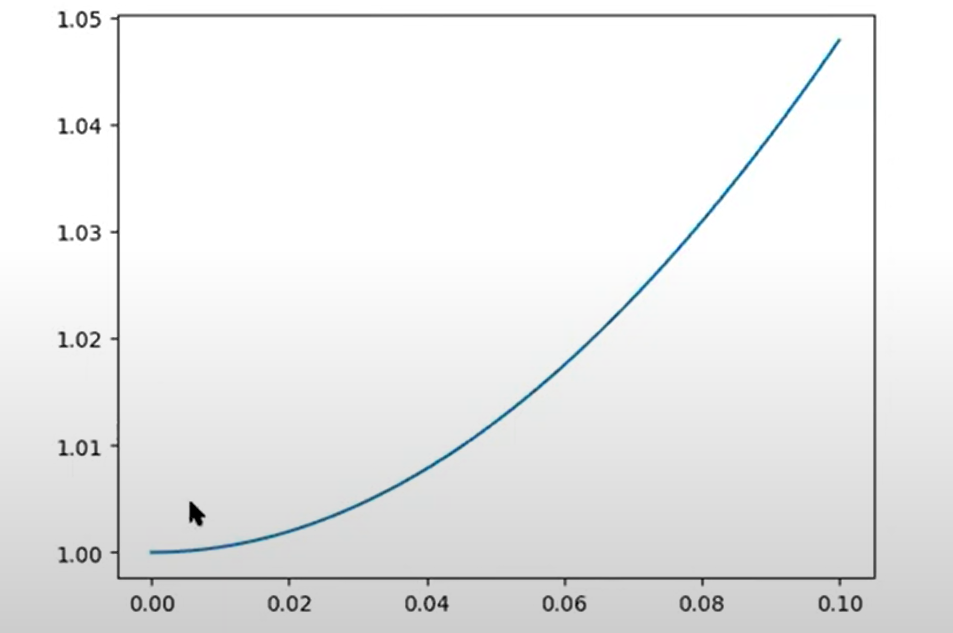
\includegraphics[width=0.4\linewidth]{L2_Images/L2_plot.PNG}
    \caption{Plot of eigenvalues versus step size.}
    \label{fig:l2f1}
\end{figure}
We see the system is marginally stable in the limit of $h \rightarrow 0$. This means that for any value of timestep $h$, the system is going to blow up!

\subsection{Take-Away Messages!}
The takeaway message from this is - 
\begin{itemize}
    \item Be careful when discretizing ODEs!
    \item Do a sanity check based on the equilibrium energy behavior (whether there is conservation and / or dissipation of energy). 
    \item This is an artifact of forward Euler integration - it always overshoots the function it is trying to approximate (in this case, it overestimates the acceleration of the system), so avoid it!
    Especially for undamped systems! 
\end{itemize}

\subsection{A better explicit integrator}
A better explicit integrator to use is the 4th order Runge-Kutta method, the ``industry standard''. The intuition of this is that Euler Integration fits a line-segment over each timestep, whereas the 4th order Runge-Kutta method (RK4) fits a cubic polynomial, which is much more expressive, and allows for much better accuracy in capturing the underlying function. 

\noindent
Here's some pseudo code for the RK4 method - 

\renewcommand{\algorithmicrequire}{\textbf{Input:}}
\renewcommand{\algorithmicensure}{\textbf{Output:}}
\algnewcommand{\LineComment}[1]{\Statex \(\triangleright\) #1}
\algnewcommand{\LineComment2}[1]{\Statex \hspace*{0.45\linewidth} \(\triangleright\) #1}
\algnewcommand{\LineComment3}[1]{\Statex \hspace*{\fill} \(\triangleright\) #1}

\\

\begin{algorithm}
	\caption{4th Order Runge-Kutta Integration}
	\label{alg:Alg1}
	\begin{algorithmic}[1]	
        \State $x_{k+1} = f_{RK4} (x_k)$
        \State $K_1 = f(x_k)$ \Comment{Evaluate at beginning.}
        \State $K_2 = f(x_k + \frac{1}{2} h K_1)$ \Comment{Evaluate at midpoint.}
        \State $K_3 = f(x_k + \frac{1}{2} h K_2)$ \Comment{Evaluate at midpoint.}
        \State $K_4 = f(x_k + h K_3)$ \Comment{Evaluate at end.}
        \State $x_{k+1} = x_{k} + \frac{h}{6} (K_1 + 2K_2 + 2K_3 + K_4)$ \Comment{Evaluate as weighted average of intermediate computations.}
	\end{algorithmic}
\end{algorithm}

\\

\noindent
Let's try this on our Pendulum example. Instead of the explosion we observed before, the eigenvalues are right within the unit circle, and reflect the true continuous system. 

\subsection{Take-Away Message!}
The 4th order Runge-Kutta method provides us with much improved accuracy, that easily outweighs the additional computational cost of 4 function evaluations instead of 1 that forward Euler integration did. 
That said, even sophisticated integrators have issues, depending on the value of timesteps, etc. So always perform some kind of sanity check! 

\section{Implicit Form}
Another thing to consider is the implicit form of an ODE. For example, the implicit form of a discrete-time dynamical system is: 
\begin{align}
    f_{\rm d} (x_{k+1}, x_{k}, u_k) = 0
\end{align}
The simplest example of this is: 
\begin{align}
    x_{k+1} = x_{k} + h f(x_{k+1}) 
\end{align}
which is \textit{Backward Euler Integration}, where we are evaluating the function $f$ at a future time. 

\noindent
How do we simulate this kind of system? 
You can write this as: 
\begin{align}
    f_{\rm d} (x_{k+1}, x_k, u_k) = x_k + h f(x_{k+1}) - x_{k+1} = 0
\end{align}
You can then treat this as a root-finding problem in $x_{k+1}$. (We'll spend time on this next week). 

\noindent
In the pendulum example, we obesrve the following - 
\begin{itemize}
    \item We see the opposite energy behavior from forward Euler integration.
    \item Discretization adds artificial damping to the system, instead of adding energy to the system. 
    \item Backward Euler undershoots the function being approximated. 
    \item While this doesn't reflect the physical process (is unphysical), this effect allows simulators to take big steps, and can be convenient sometimes!
    \item It is very common to use this in quick and easy low-fi simulators in graphics and robotics. 
\end{itemize}

\subsection{Take-Away Message!}
\begin{itemize}
    \item Implicit methods are often ``more stable'' than their explicit counterparts. 
    \item For forward simulation, solving the implicit equation can be more expensive. 
    \item In many ``direct'' trajectory optimization methods, they are \textit{not} any more expsensive to use! 
\end{itemize}

\section{Discretizing Controls}
So far, we've focused on discretizing the state of the system $x(t)$. We also have the control input to the system, $u(t)$ that we need to discretize!

\noindent
The simplest option here is to set: 
\begin{align}
    u(t) = u_k  \ t_{k} \leq t \leq t_{k+1} 
\end{align}
This is a ``zero-order hold'', where the control input at time $t$ is simply equal to the control input within the corresponding time interval. This is a piecewise constant control. 
This is easy to implement, but may require lots of knot points (sample points) to accurately capture a continuous control input $u(t)$.

\noindent
There are possibly better options, such as:
 \begin{align}
     u(t) = u_{k} + \frac{u_{k+1}-u_k}{h} (t-t_n)
 \end{align}
This is a ``first order hold'', or a piecewise \textit{linear} control. The control input is a linear function of the control inputs at the end points of the time interval. 
This first-order hold can better approximate continuous $u(t)$ with fewer knot points, thus leading to faster solve times, etc. It's not too much more work than the zero-order hold computationally speaking. If you know your system is continuous, use the first order hold! 
It's also very common to do this, such as classic DIRCOL (direct collocation). 

\noindent
There are other options too - 
\begin{itemize}
    \item We can progressively move to higher-order holds, using higher-order polynomials. 
    \item In many control applications, $u(t)$ is \textit{not} smooth, such as in bang-bang control methods. In these cases, higher-order polynomials are not the best choice, and are not good approximations. 
\end{itemize}

\noindent
In general, zero-order and first-order holds are the most common ways to discretize control in practice.


